\chapter{Introduction}
\label{sec:introduction}

Since the invention of modern computers Monte Carlo methods have become an frequently applied tool for challenging numerical problems in a wide variety of fields ranging from chemical physics to financial econometrics. Although the evolution of computers is proceeding, the complexity of the treated problems is growing faster and Monte Carlo methods are now expected to deal with high dimensionalities and more and more complex structures. Hence, the computational complexity of these methods is nowadays a crucial question.

Whereas Monte Carlo methods build a broad class of computational algorithms that generally rely on the principle of repeated random sampling to solve a numerical problem, the Markov chain Monte Carlo (MCMC) methodology~\autocite{Robert2005} provides a framework for many algorithms which perform the sampling from complex probability distributions in high dimensions by generating a Markov chain, which has the desired probability distribution as its equilibrium distribution. In many situations, this is a suitable and efficient strategy to solve emergent problems in applications~\autocite{Liu2004, Robert2005}. It is therefore of interest to analyze the structure inherent to these algorithms to understand their computational complexity. This is most naturally undertaken by studying the behavior of the method on a family of probability distributions indexed by a parameter and then studying the cost of the algorithm as a function of that parameter. As a fruitful way to do this, the theory of  diffusion limits for MCMC methods in high dimensions is an established approach and provides a useful theoretical tool for studying computational complexity. In particular we will study these algorithms applied to different classes of probability distributions, i.e., distributions found from finite-dimensional approximations of a measure on an infinite-dimensional space. This setting arises in widely used applications such as Bayesian nonparametric statistics or conditioned diffusion~\autocite{Beskos2008, Beskos2009, Dashti2012, Dashti2013, Delyon2006, Hairer2011, Stuart2010}.
\newline

Our interest is focused on Metropolis-Hastings MCMC methods. We study the Random Walk Metropolis algorithm (RWM) and the Metropolis-adjusted Langevin algorithm (MALA)~\autocite{Liu2004, Robert2005}. The Metropolis-Hastings~(MH) methodology is simple but effectiv. To generate samples from a $N$-dimensional target density $ \pi^{N} $, a Markov chain according to a random walk is constructed. As it is complicated, to build a chain which is invariant for~$\pi^N$ in the first attempt, a two-step algorithm is used. First,  a candidate according to an arbitrary transition rule is generated. In a second step, this candidate or proposal is rejected with a certain probability such that the so generated Markov chain will be $\pi^N$-invariant. While the second acceptance-rejection step, often called 'Metropolizing' is fixed, the choice of an suitable proposal is free. Two widely used proposals are the random walk proposal (obtained from
the discrete approximation of Brownian motion)
\begin{equation}
\label{RWM-proposals-simple} 
  y = x + \sqrt{2\delta}\,Z^{N}, \qquad Z^{N} \thicksim \mathcal{N}\left( 0,I_N \right),
\end{equation}

and the Langevin proposal (obtained from the time discretization of the
Langevin diffusion)
\begin{equation}
\label{MALA-proposals-simple}
  y = x +  \delta \nabla \log \pi^{N} (x) + \sqrt{2\delta} Z^N, \qquad Z^{N} \thicksim \mathcal{N}\left( 0,I_N \right).
\end{equation}

Here $ 2 \delta $ is the proposal variance, a parameter quantifying the size of the discrete time increment; we will consider “local proposals” for which $ \delta $ is
small and note that $ \delta $ will depend on the dimension $N$, i.e. $\delta  = \delta(N) $. The Equations~(\ref{RWM-proposals-simple}) and~(\ref{MALA-proposals-simple}) can be expressed in terms of transition kernels~$q(x,y)$. Now, through Metropolizing some candidates are rejected according to the following rule: from the current state $ x $, we propose $ y $ drawn from the kernel $ q(x, y) $; this is then accepted with probability
\begin{equation}
\label{acceptance probability simple}
 \alpha^{N}(x,y)  := 1 \wedge \dfrac{\pi^{N}(y) q(y,x) }{\pi^{N}(x) q(x,y)}
\end{equation}
and otherwise rejected. Here $ a \wedge b := \min (a,b)$. The Markov chain corresponding to proposal given in Equation~(\ref{RWM-proposals-simple}) is the (RWM) algorithm~\autocite{Metropolis1953}, and the Markov transition rule constructed from the proposal defined in Equation~(\ref{MALA-proposals-simple}) is known as the (MALA) algorithm~\autocite{Robert2005}.

\begin{figure}%[htb]
 \begin{center} 
  \includegraphics[width=0.6\textwidth]{figure_1}
  \vspace*{1mm}
  \subcaption{'Optimal scaled' RWM algorithm with a good mixing between both modes.}
  \label{fig:3DscatterplotRWM-optimal}
  \vspace*{3mm}
  \includegraphics[width=0.6\textwidth]{figure_2}
  \vspace*{1mm}
  \subcaption{Too small proposal variance with strong dependences.}
  \label{fig:3DscatterplotRWM-small}
  \vspace*{3mm}
  \includegraphics[width=0.6\textwidth]{figure_3}
  \vspace*{1mm}
  \subcaption{Too large proposal variance causes too much rejected movements.}
  \label{fig:3DscatterplotRWM-large}
 \end{center}
  \caption{5000 samples produced by a RWM algorithm of a multimodal non-product target density. 1000 consecutive samples are always labeled in the same color.}
  \label{fig:3DscatterplotRWM}
\end{figure}

Let us now consider an heuristic argument for an optimal scaling of these Metropolis-Hastings algorithm via the proposal variance~$\delta(N)$. In Figure~\ref{fig:3DscatterplotRWM}, the optimal scaling characteristic of Metropolis-Hastings methods is illustrated by a Random Walk Metropolis-Hastings algorithm. The first 5000 samples produced by a RWM algorithm applied to a multimodal non-product target measure in dimension $N=10$ are depicted. Thereby every 1000 consecutive samples are labeled in the same color to better illustrate the movement of the generated chain. These sample chains generated by the RWM (or MALA) algorithm should ideally be not correlated, as strong dependences in the samples leads to poorer MCMC estimates. Hence good mixture of the colors in Figure~\ref{fig:3DscatterplotRWM} visualizes fewer dependences between the samples and vice versa. 

\begin{figure}[htb]
\begin{center}
  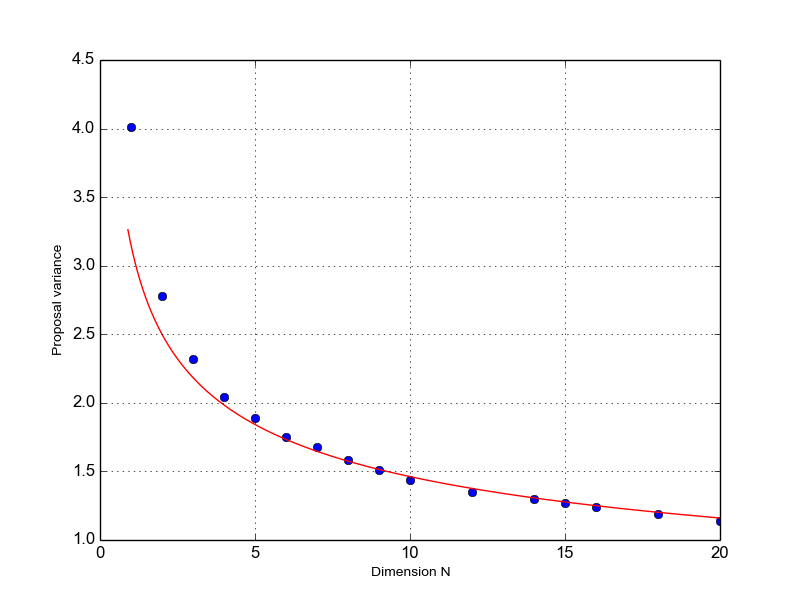
\includegraphics[width=0.65\textwidth]{proposalvariancesForDimensions}
\end{center}
  \caption{Proposal variances~$\delta$ for a MALA algorithm applied to a standard Gaussian distribution such that the mean average acceptance rate~$\alpha$ of the simulation is approximately 0.50 (blue). As comparison, the function $F(N) = 3.15 \; N^{-1/3}$ is given (red).}
  \label{fig:proposalVarianceForDimensions}
\end{figure}

A simple numerical simulation as in Figure~\ref{fig:3DscatterplotRWM} illustrates that too small or large proposal variances make the performance of the algorithm arbitrarily poor. For extremely small proposal variances, see Figure~\ref{fig:3DscatterplotRWM-small}, the algorithm will propose only small jumps and almost every step will be accepted. Therefore the average acceptance rate is almost one. However, the size of the proposed jumps is too small to explore the target distribution rapidely. The convergence of the algorithm to its stationary distribution will take too long. In the case of a too large proposal variances, the algorithm will propose large jumps (to far distant regions). It will therefore reject most of its proposed moves and the Markov chain stays in single states for a long period of time. It seems reasonable that there exist 'good' intermediate values for the proposal variance (see Figure~\ref{fig:3DscatterplotRWM-optimal}). This behavior is observable for every dimension $N$.

Moreover, such 'optimal' intermediate proposal variances $ \delta(N) $ seems to decrease with increasing dimension $N$. In Figure~\ref{fig:proposalVarianceForDimensions}, we have applied the MALA algorithm to a standard Gaussian distribution in different dimensions~$N$ and plotted the proposal variance~$\delta$ such that the mean acceptance probability for 10,000 iterations is approximately 0.50. To have a better comparison, we plotted the function $F(N) = 3.15 \; N^{-1/3}$ in the same diagram. The scaling~$N^{- 1/3}$ is shown to be optimal for product measures such as Gaussian measures in previous works~\autocite{Roberts1997, Roberts1998}. A similar behavior can be observed for nonproduct measures.

\subsection*{Statement of the problem}

The structure of the Metropolis-Hastings methods introduced above is rather simple. At each step a move is proposed according to Equation~(\ref{RWM-proposals-simple}) or~(\ref{MALA-proposals-simple}) and this candidate is accepted with a certain probability given in Equation~(\ref{acceptance probability simple}). These quantities depend on the target distribution $ \pi^{N} $ and the proposal kernel $ q(x,y) $, which is characterized by the proposal variance $ \delta(N) $ in the case of Gaussian jumps. Hence all occurring quantities can be indexed by a parameter; in this case the dimension $N$. Our aim is to study the cost as a function of dimension for the RWM and MALA algorithm applied to different families of probability distributions. Early results~\autocite{Roberts1997, Roberts1998} concerned product measures for which an optimal scaling via diffusion limits for RWM and MALA was obtained. It was shown that the computational complexity of RWM started in stationarity and applied to simple product distributions is $\mathcal{O}(N)$ for an average acceptance rate of 0.234~\autocite{Roberts1997}. Similarly, the cost of MALA, started in stationarity and applied to simple product distributions was characterized by $\mathcal{O}(N^{1/3})$ for an average acceptance rate of 0.573~\autocite{Roberts1998}. 

In this work, we want to summarize the results of Mattingly, Pillai and Stuart~\autocite{Mattingly2010} and Pillai, Stuart and Thi\'{e}ry~\autocite{Pillai2012}. They proved that the optimal scaling of RWM and MALA as mentioned above holds for finite-dimensional approximations of measures obtained from Gaussian measures in infinite dimensional Hilbert spaces by a change of measures. This specific setting occurs in widely used applications such as Bayesian nonparametric statistics with Gaussian priors and conditioned diffusion with additive noise~\autocite{Beskos2009, Stuart2010}.

More precisely, we will combine and summarize the methods from~\autocite{Mattingly2010} and~\autocite{Pillai2012} to prove a diffusion limit result for RWM and MALA in the above Hilbert space setting simultaneously, where the speed of the interpolant of the generated Markov chains and the proposal variance of the RWM or MALA candidates scales in the correct sense. This diffusion limit result enables us to quantify the computational cost or efficiency uniquely. On the other hand this statement holds only asymptotically. As we will see in Chapter~\ref{Numerical Results} that it seems reasonable for these asymptotic results to hold for finite dimensions, too. This point of view is supported by several numerical studies~\autocite{Beskos2008, Gelman1996, Roberts2001}.



\subsection*{Own contributions}

My contributions to the present topic.
\begin{itemize}
 \item Combining and resuming the proof (strategy) of Mattingly, Pillai and Stuart~\autocite{Mattingly2010} and Pillai, Stuart and Thi\'{e}ry~\autocite{Pillai2012}.
 \item Give a comprehensive overview.
 \item Numerical studies.
\end{itemize}


\subsection*{Outline}

In Chapter~\ref{sec:Metropolis-HastingsMethod} we will introduce the Metropolis-Hastings methodology rigorously. Especially, convergence and ergodicity properties of the general Metropolis-Hastings algorithm are presented. Additionaly, the two frequently used variants of the MH algorithm, the Random Walk Metropolis algorithm and the Metropolis adjusted Langevin algorithm are described. Chapter~\ref{ch:Computational Complexity} comprises a brief introduction in the theory of computational complexity and describes different ways to measure complexity in the case of MCMC methods. This will us allow to scale the algorithm in such a way that the complexity is minimal. Such a scale we will call optimal. To complete the picture of complexity, we give an overview on existing optimal scaling results for the RWM and MALA algorithm. In Chapter~\ref{Application} two main applications of the RWM and MALA algorithm are given: conditioned diffusions and Bayesian nonparametric statistics. Chapter~\ref{Diffusion Limit Results} contains statement and proof of the main theorem of this work. According to Mattingly, Pillai and Stuart~\autocite{Mattingly2010} and Pillai, Stuart and Thi\'{e}ry~\autocite{Pillai2012}, we state a diffusion limit result indicating that the optimal scaling of RWM and MALA  for target distributions found from finite-dimensional approximations of a measure on an infinite-dimensional Hilbert space is $\mathcal{O}(N)$ and $\mathcal{O}(N^{1/3})$, respectively. Finally, Chapter~\ref{Numerical Results} gives a numerical study suggesting that the asymptotic results in the previous chapters hold in finite dimensions.


\subsection*{Acknowledgements}

A list of persons, who deserve my acknowledgements: advisor, parents, friends.



